%%=============================================================================
%% Onderzoek
%%=============================================================================

\chapter{Onderzoek}
\label{ch:onderzoek}

\section{Methodologie}
\label{sec:methodologie}

\subsection{Opzetten microservices}
\label{sec:opzetten}

De opstelling kent de volgende microservices:
\begin{itemize}
\item eureka: service discovery
\item zipkin: Zipkin server voor tracing
\item ms-web: Spring Boot app die root microservice voorstelt
\item ms-service-n: Spring Boot app voor bijkomende microservices (n staat voor een cijfer van 1 t.e.m. 27)
\end{itemize}

Dit onderzoekt bekijkt drie verschillende opstellingen, geonderscheid op complexiteit, om de tracing performantie na te gaan. De setup met lage complexiteit kent in totaal 4 microservices en 2 niveau's.
\begin{figure}[h]
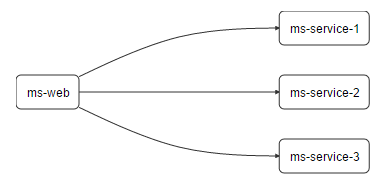
\includegraphics{ms_lc_dependencies}
\end{figure}
De setup met gemiddelde complexiteit kent 11 microservices en 3 niveau's.
\begin{figure}[h]
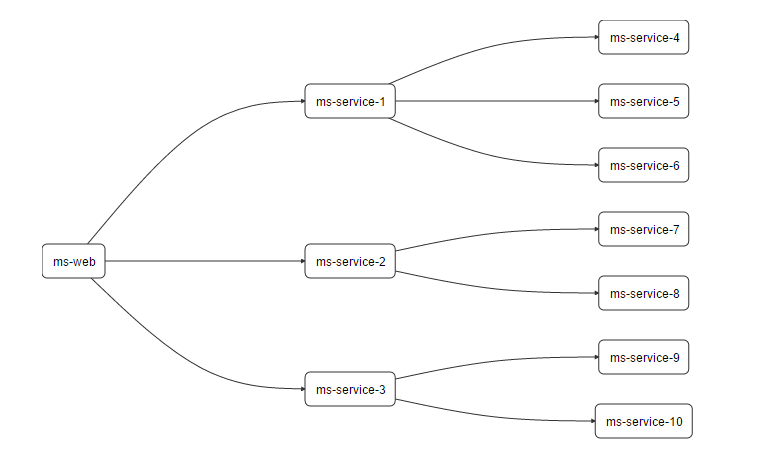
\includegraphics[scale=0.5]{ms_dependencies}
\end{figure}
De setup met hoge complexiteit kent 28 microservices en 4 niveau's. 
\begin{figure}[h]
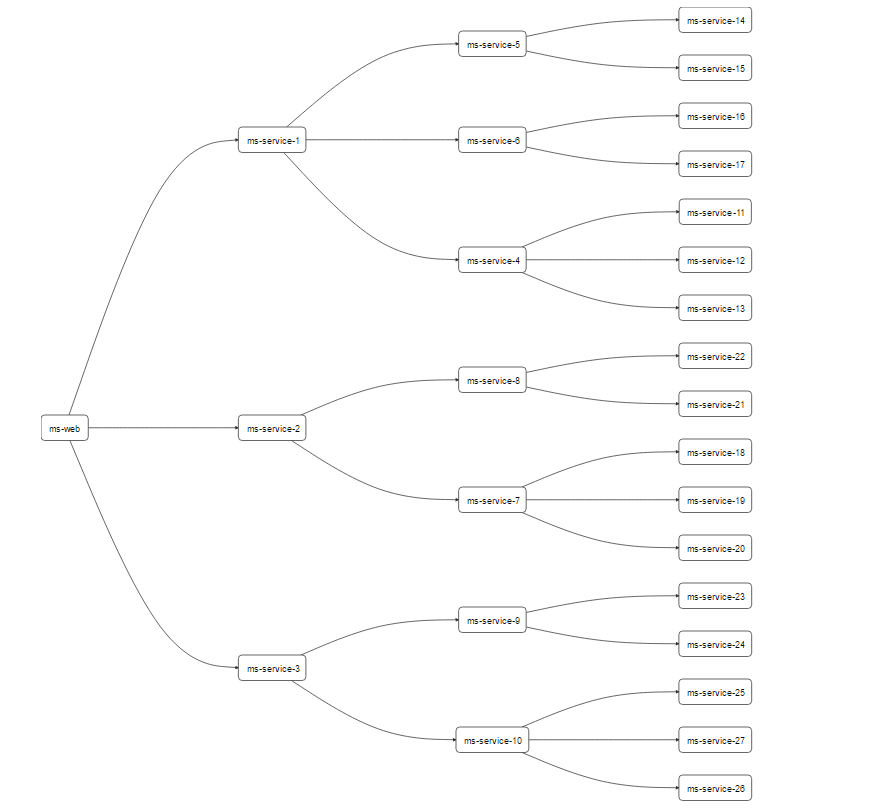
\includegraphics[scale=0.5]{ms_hc_dependencies}
\end{figure}

De Spring Cloud Sleuth bibliotheek wordt toegevoegd aan de ms-web en ms-service-n microservices, zodat deze services tracing info doorsturen naar de zipkin server.

Elke microservice krijgt zijn eigen Docker container, die allemaal tegelijk worden opgestart met Docker Compose, dankzij het toevoegen van een docker-compose.yml script (bijlage) die alle service definities bevat.

De microservices communiceren asynchroon met elkaar, zodat de ene service niet hoeft te wachten op de andere. Dit verbetert de responstijd. Vergelijk figuur \ref{fig:sync_rest} met figuur \ref{fig:async_rest}.

\begin{figure}
\caption{Synchrone REST calls tussen microservices, gevisualiseerd in Zipkin}
\centering
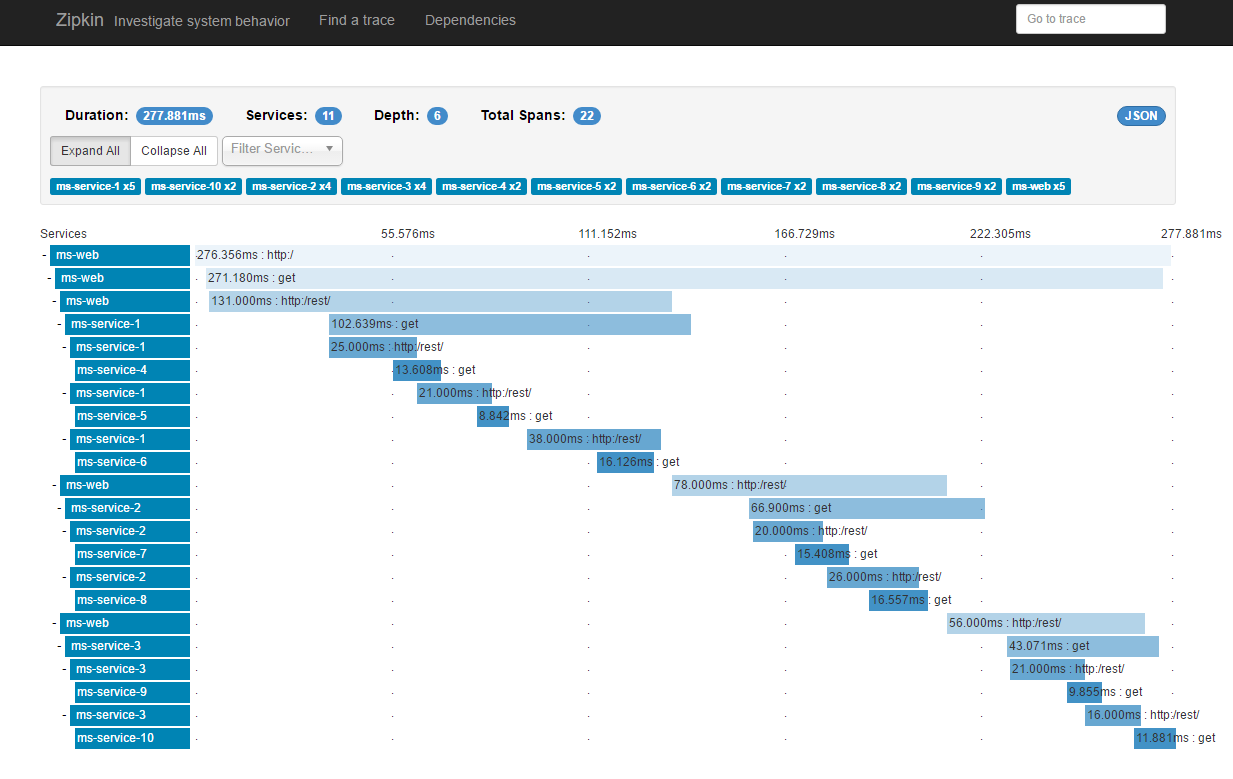
\includegraphics[width=1\textwidth]{sync_traces_zipkin}
\label{fig:sync_rest}
\end{figure}

\begin{figure}
\caption{Asynchrone REST calls tussen microservices, gevisualiseerd in Zipkin}
\centering
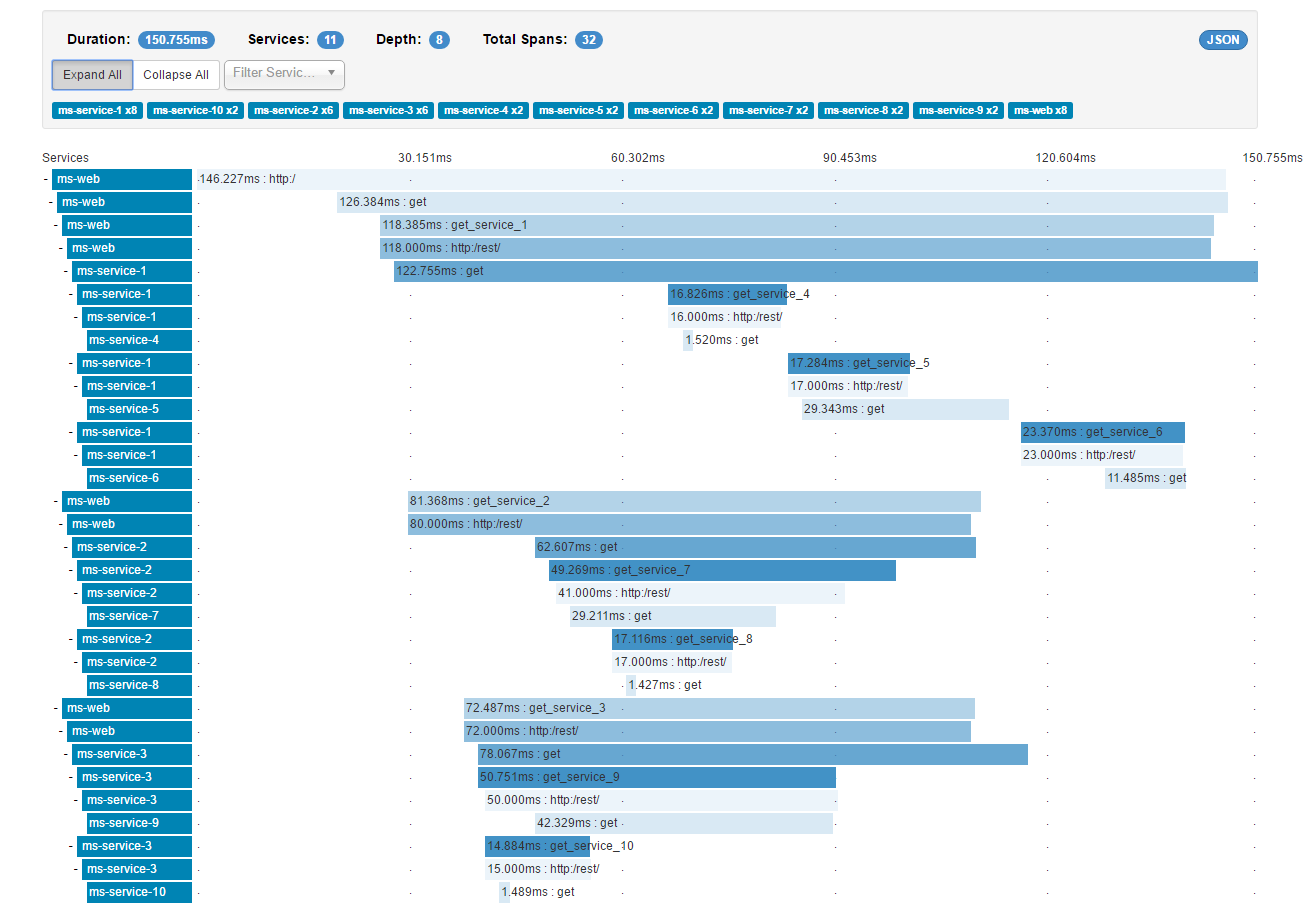
\includegraphics[width=1\textwidth]{async_traces_zipkin}
\label{fig:async_rest}
\end{figure} 

Om de asynchrone communicatie tussen services mogelijk te maken wordt gebruik gemaakt van \texttt{ListenableFuture} van guava (Google Core libraries voor Java) in combinatie met \texttt{TraceCallable} van Sleuth. \texttt{TraceCallable} is een wrapper van Sleuth voor een Java \texttt{Callable} die tracing informatie toevoegt. Een gewone \texttt{Callable} voert een taak uit op een andere thread en geeft een resultaat terug.

\begin{lstlisting}[language=Java, basicstyle=\ttfamily\scriptsize, caption=Asynchrone REST communicatie]
@RestController
@RequestMapping("/")
public class SimpleRestController {
    private static final ListeningExecutorService executor = MoreExecutors.listeningDecorator(Executors.newCachedThreadPool());
    
    @Autowired
    private RestTemplate restTemplate;

    @Autowired
    private Tracer tracer;

    @Autowired
    private SpanNamer spanNamer;

    @RequestMapping(method = RequestMethod.GET)
    public String get() throws ExecutionException, InterruptedException {
        Callable<ResponseEntity<String>> callable1 = new Callable<ResponseEntity<String>>() {
            @Override
            public ResponseEntity<String> call() throws Exception {
                return requestService("http://ms-service-1:8080/rest/");
            }
        };
        Callable<ResponseEntity<String>> traceCallable1 = new TraceCallable<>
                (tracer, spanNamer, callable1, "get_service_1");

        ListenableFuture<ResponseEntity<String>> future1 = executor.submit(traceCallable1);

        ...

        // wait for results
        ResponseEntity<String> service1Response = future1.get();
        
        ...
        
        return serviceResponse.getBody();
    }

    private ResponseEntity<String> requestService(String serviceUrl) {
        return restTemplate.exchange(serviceUrl, HttpMethod.GET, null, String.class);
    }

}
\end{lstlisting}

Een \texttt{Tracer} en een \texttt{SpanNamer} worden geïnjecteerd door Sleuth en een \texttt{RestTemplate} door Spring. Omdat Sleuth automatisch tracing informatie toevoegt aan een \texttt{RestTemplate}, moet dit niet verder geconfigureerd worden.

\subsection{Sampling strategieën en performantieverschillen}
\label{sec:sampling}

Er wordt onderzocht wat voor overhead het toevoegen van tracing informatie met zich meebrengt op de drie verschillende testopstellingen (zie \ref{sec:opzetten}). Omdat Sleuth gebaseerd is op Dapper, wordt bekeken hoe verschillende sampling strategieën de performantie beïnvloeden. Uit \autocite{Sigelman2010} blijkt immers dat verzameling van traces de grootste invloed kan hebben op vertragingen in het netwerk bij het maken van requests.

Met een gesampelde trace wordt bedoeld dat de trace gemarkeerd is om verzameld te worden. In dit onderzoek betekent dit dat Sleuth een gesampelde trace zal doorsturen naar de Zipkin server. Om de sampling te definiëren voor een bepaalde service dient een Java bean aangemaakt te worden. Sleuth zal deze Sampler automatisch opmerken en gebruiken. Om bijvoorbeeld alle requests te tracen, kan gebruik gemaakt worden van Sleuth's \texttt{AlwaysSampler}.

Om slechts een percentage van de requests te tracen, kan een eigen sampler gedefinieerd worden als volgt:

\begin{lstlisting}[language=Java, basicstyle=\ttfamily\small, caption=Sleuth percentage sampler]
@Bean
public Sampler percentageSampler() {
    return new Sampler() {
        @Override
        public boolean isSampled(Span span) {
            Random rg = new Random();
            // trace 50% of all requests
            return rg.nextInt(10) > 4;
        }
    };
}
\end{lstlisting}

Dit onderzoek gaat na welke performantiegevolgen verschillende sampling percentages op de verschillende gedefinieerde microservice opstellingen (zie \ref{sec:opzetten}) hebben. Er wordt gebruik gemaakt van de Apache Benchmark (ab) tool om de responstijd te testen. Bij de testen wordt rekening gehouden met een \textit{concurrency} variabele, dat aanduidt hoeveel requests er tegelijk worden uitgevoerd. Voor een hoog netwerkverkeer te simuleren worden er 1000 requests tegelijk uitgevoerd tot er 10 000 requests in totaal aangekomen zijn. De bovenlimiet 1000 is gekozen, omdat dit het maximaal aantal verbindingen is dat het gebruikte testsysteem tegelijk toelaat. Een gemiddeld netwerkverkeer wordt gesimuleerd door 200 requests tegelijk uit te voeren tot alweer 10 000 requests verwerkt zijn en een laag netwerkverkeer zal ten slotte 20 requests tegelijk uitvoeren.

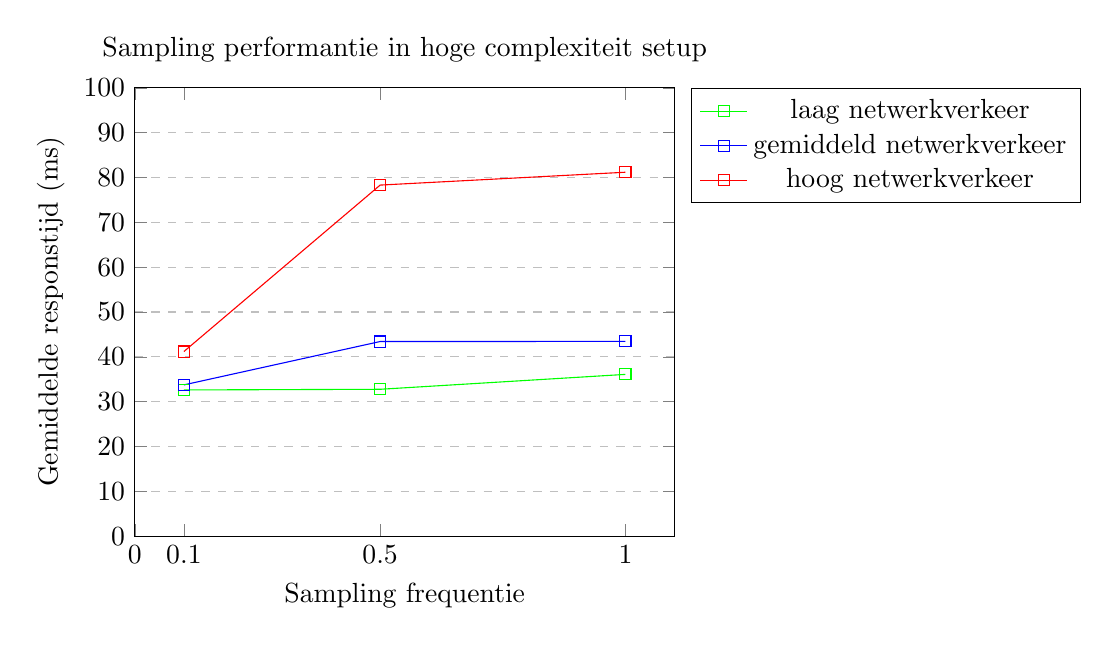
\begin{tikzpicture}
\begin{axis}[
    title={Sampling performantie in hoge complexiteit setup},
    xlabel={Sampling frequentie},
    ylabel={Gemiddelde responstijd (ms)},
    xmin=0, xmax=1.1,
    ymin=0, ymax=100,
    xtick={0, 0.1, 0.5, 1},
    ytick={0, 10, 20, 30, 40, 50, 60, 70, 80, 90, 100},
    %xticklabel style={/pgf/number format/.cd,frac,frac TeX=\displaystyle\frac},
    legend pos=outer north east,
    ymajorgrids=true,
    grid style=dashed,
    xlabel near ticks,
    ylabel near ticks
]
 
\addplot[
    color=green,
    mark=square,
    ]
    coordinates {(0.1,32.621)(0.5,32.769)(1,36.091)};
    
\addplot[
    color=blue,
    mark=square,
    ]
    coordinates {(0.1,33.752)(0.5,43.422)(1,43.45)};
    
\addplot[
    color=red,
    mark=square,
    ]
    coordinates {(0.1,41.192)(0.5,78.317)(1,81.184)};

\addlegendentry{laag netwerkverkeer}
\addlegendentry{gemiddeld netwerkverkeer}
\addlegendentry{hoog netwerkverkeer}
\end{axis}
\end{tikzpicture}

Voor de hoge complexiteit setup blijkt dat tracing vanaf 50\% sampling frequentie en bij hoog netwerkverkeer een grote stijging kent in responstijd ten opzichte van de responstijd bij 10\% sampling. De responstijd stijgt van 41,2 ms naar 78,3 ms voor 50\% sampling en 81,2 ms voor 100\% sampling.

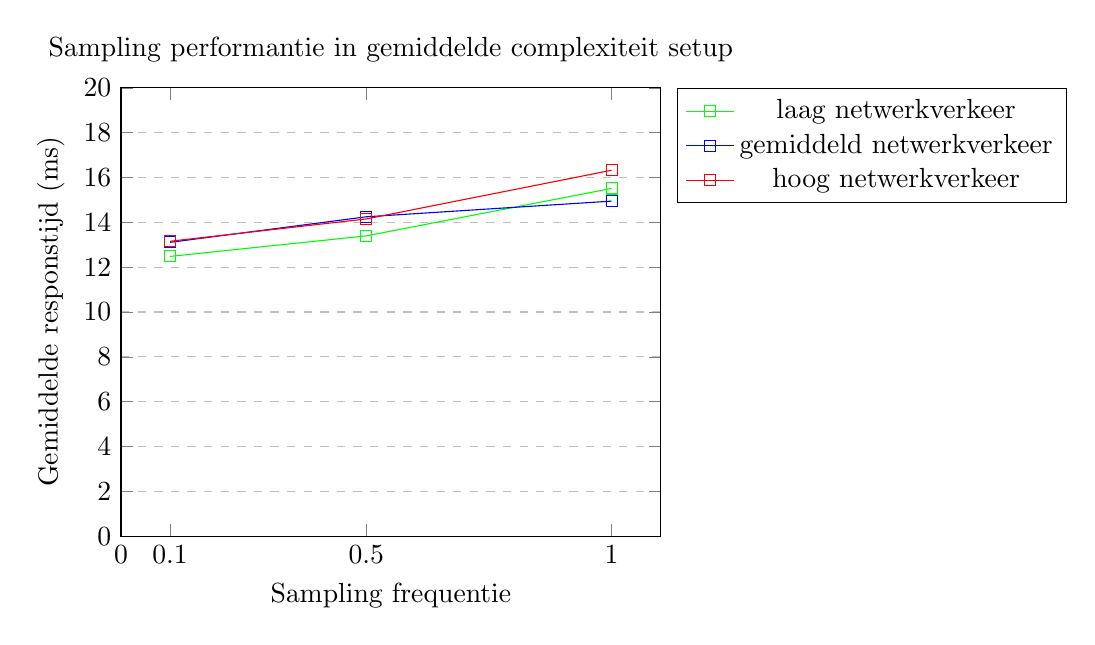
\begin{tikzpicture}
\begin{axis}[
    title={Sampling performantie in gemiddelde complexiteit setup},
    xlabel={Sampling frequentie},
    ylabel={Gemiddelde responstijd (ms)},
    xmin=0, xmax=1.1,
    ymin=0, ymax=20,
    xtick={0, 0.1, 0.5, 1},
    ytick={0, 2, 4, 6, 8, 10, 12, 14, 16, 18, 20},
    %xticklabel style={/pgf/number format/.cd,frac,frac TeX=\displaystyle\frac},
    legend pos=outer north east,
    ymajorgrids=true,
    grid style=dashed,
    xlabel near ticks,
    ylabel near ticks
]
 
\addplot[
    color=green,
    mark=square,
    ]
    coordinates {(0.1,12.482)(0.5,13.398)(1,15.514)};
    
\addplot[
    color=blue,
    mark=square,
    ]
    coordinates {(0.1,13.109)(0.5,14.249)(1,14.948)};
    
\addplot[
    color=red,
    mark=square,
    ]
    coordinates {(0.1,13.158)(0.5,14.153)(1,16.325)};

\addlegendentry{laag netwerkverkeer}
\addlegendentry{gemiddeld netwerkverkeer}
\addlegendentry{hoog netwerkverkeer}
\end{axis}
\end{tikzpicture}

...

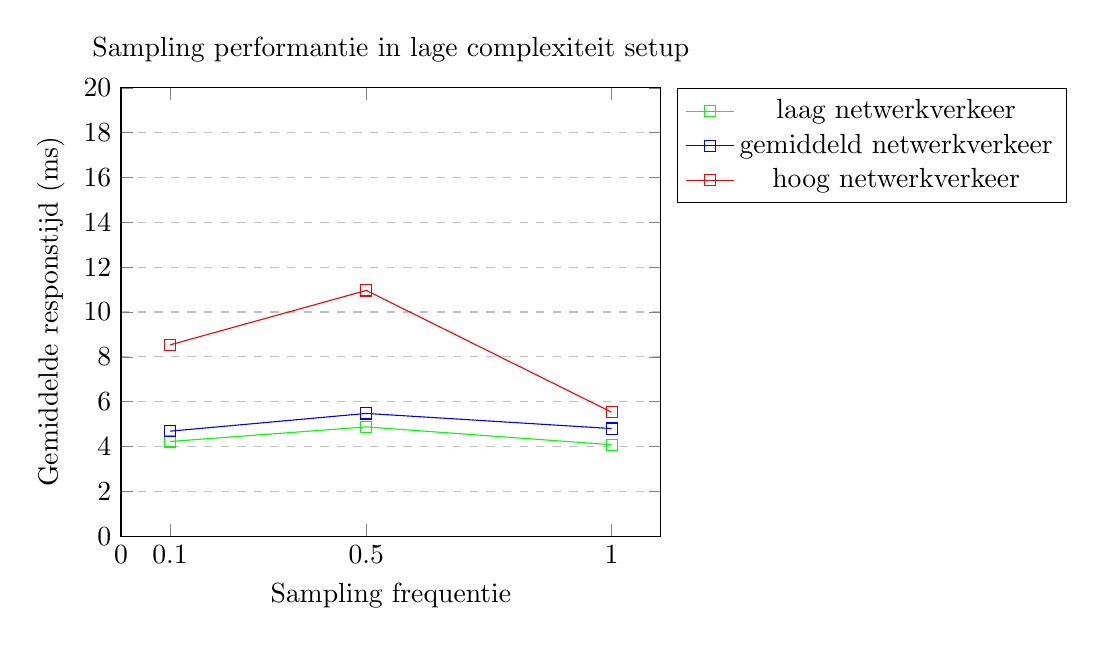
\begin{tikzpicture}
\begin{axis}[
    title={Sampling performantie in lage complexiteit setup},
    xlabel={Sampling frequentie},
    ylabel={Gemiddelde responstijd (ms)},
    xmin=0, xmax=1.1,
    ymin=0, ymax=20,
    xtick={0, 0.1, 0.5, 1},
    ytick={0, 2, 4, 6, 8, 10, 12, 14, 16, 18, 20},
    %xticklabel style={/pgf/number format/.cd,frac,frac TeX=\displaystyle\frac},
    legend pos=outer north east,
    ymajorgrids=true,
    grid style=dashed,
    xlabel near ticks,
    ylabel near ticks
]
 
\addplot[
    color=green,
    mark=square,
    ]
    coordinates {(0.1,4.225)(0.5,4.875)(1,4.08)};
    
\addplot[
    color=blue,
    mark=square,
    ]
    coordinates {(0.1,4.685)(0.5,5.477)(1,4.802)};
    
\addplot[
    color=red,
    mark=square,
    ]
    coordinates {(0.1,8.535)(0.5,10.964)(1,5.531)};

\addlegendentry{laag netwerkverkeer}
\addlegendentry{gemiddeld netwerkverkeer}
\addlegendentry{hoog netwerkverkeer}
\end{axis}
\end{tikzpicture}

...

\subsection{Logging}

...